\batchmode
\documentclass[11pt]{article}
\RequirePackage{ifthen}


\usepackage{graphics,graphicx}

\DeclareGraphicsExtensions{.ps,.jpg,.eps,.pdf,.png} 
\usepackage{boxedminipage,amsmath,amsfonts}
\usepackage{url}
\usepackage{verbatim,moreverb}
\bibliographystyle{plain}

%
\providecommand{\figurepath}{./figures}%
\providecommand{\bibpath}{/Users/kmartin/Documents/files/misc}%
\providecommand{\figfiletype}{pdf} 

%
\providecommand{\T}{ {\rm T} }%
\providecommand{\R}{ {\bf R} }%
\providecommand{\C}{ {\bf C} }%
\providecommand{\D}[2]{ \frac{\partial #1}{\partial #2} }%
\providecommand{\DD}[3]{ \frac{\partial^2 #1}{\partial #2 \partial #3} }%
\providecommand{\Dpow}[2]{ \frac{\partial^{#1}}{\partial  {#2}^{#1}} }%
\providecommand{\dpow}[2]{ \frac{ {\rm d}^{#1}}{{\rm d}\, {#2}^{#1}} } 



%
\newenvironment{hangref}{\begin{list}{}{\setlength{\itemsep}{4pt}
  \setlength{\parsep}{0pt}\setlength{\leftmargin}{+\parindent}
  \setlength{\itemindent}{-\parindent}}}{\end{list}} 


\marginparwidth 0pt\marginparsep 0pt \topskip 0pt\headsep
0pt\headheight 0pt \oddsidemargin 0pt\evensidemargin 0pt
\textwidth 6.5in \topmargin 0pt\textheight 9.0in

\newtheorem{theorem}{Theorem} 


\newcounter{Fig} %
\renewcommand{\theFig}{\arabic{Fig}}%
\providecommand{\Fig}[2]{\refstepcounter{Fig} \label{#1}
                     {\small\bf Figure \theFig .} {\small\sl #2 

}} 


\setcounter{topnumber}{3}
%
\renewcommand{\topfraction}{.9}
\setcounter{bottomnumber}{3}
%
\renewcommand{\bottomfraction}{.9}
\setcounter{totalnumber}{4}
%
\renewcommand{\textfraction}{.1}

\setlength{\floatsep}{.25in} 

\setlength{\intextsep}{.25in} 



\setlength{\fboxrule}{2\fboxrule}  
\setlength{\fboxsep}{3\fboxsep} 

%
\providecommand{\Sa}{8pt}%
\providecommand{\Sb}{0pt} 


%
\renewcommand{\_}{{\char"5F}}
%
\renewcommand{\{}{{\char"7B}}
%
\renewcommand{\}}{{\char"7D}}
%
\renewcommand{\^}{{\char"0D}}


\let\accute= \' 
%
\renewcommand{\'}{{\char"0D}}

%
\providecommand{\bfit}{\bfseries\itshape} 



\newlength{\extopskip}  
\newlength{\exbottomskip} 

\setlength{\exbottomskip}{1\baselineskip} 

\addtolength{\exbottomskip}{-5.0pt} 

\setlength{\extopskip}{1\exbottomskip} 

\addtolength{\extopskip}{-1\parskip} 



%
\newenvironment{Example}{\vspace{1\extopskip}\noindent\hspace*{2em}
                         \frenchspacing\small
                         \tt\begin{tabular}{@{}l@{}}}{
                         \end{tabular}\\[1\exbottomskip]} 

%
\providecommand{\Titem}{\item[$\triangleright$]}%
\providecommand{\Ditem}{\item[$\diamond$]} 



%
\newenvironment{Itemize}{\begin{quote}\normalsize
   \baselineskip 20pt plus .3pt minus .1pt \begin{itemize}}
   {\end{itemize}\end{quote}} 
   % Set path to folder containing figures%
\providecommand{\FigureFolder}{figures} 




\usepackage[dvips]{color}


\pagecolor[gray]{.7}

\usepackage[latin1]{inputenc}



\makeatletter

\makeatletter
\count@=\the\catcode`\_ \catcode`\_=8 
\newenvironment{tex2html_wrap}{}{}%
\catcode`\<=12\catcode`\_=\count@
\newcommand{\providedcommand}[1]{\expandafter\providecommand\csname #1\endcsname}%
\newcommand{\renewedcommand}[1]{\expandafter\providecommand\csname #1\endcsname{}%
  \expandafter\renewcommand\csname #1\endcsname}%
\newcommand{\newedenvironment}[1]{\newenvironment{#1}{}{}\renewenvironment{#1}}%
\let\newedcommand\renewedcommand
\let\renewedenvironment\newedenvironment
\makeatother
\let\mathon=$
\let\mathoff=$
\ifx\AtBeginDocument\undefined \newcommand{\AtBeginDocument}[1]{}\fi
\newbox\sizebox
\setlength{\hoffset}{0pt}\setlength{\voffset}{0pt}
\addtolength{\textheight}{\footskip}\setlength{\footskip}{0pt}
\addtolength{\textheight}{\topmargin}\setlength{\topmargin}{0pt}
\addtolength{\textheight}{\headheight}\setlength{\headheight}{0pt}
\addtolength{\textheight}{\headsep}\setlength{\headsep}{0pt}
\setlength{\textwidth}{349pt}
\newwrite\lthtmlwrite
\makeatletter
\let\realnormalsize=\normalsize
\global\topskip=2sp
\def\preveqno{}\let\real@float=\@float \let\realend@float=\end@float
\def\@float{\let\@savefreelist\@freelist\real@float}
\def\liih@math{\ifmmode$\else\bad@math\fi}
\def\end@float{\realend@float\global\let\@freelist\@savefreelist}
\let\real@dbflt=\@dbflt \let\end@dblfloat=\end@float
\let\@largefloatcheck=\relax
\let\if@boxedmulticols=\iftrue
\def\@dbflt{\let\@savefreelist\@freelist\real@dbflt}
\def\adjustnormalsize{\def\normalsize{\mathsurround=0pt \realnormalsize
 \parindent=0pt\abovedisplayskip=0pt\belowdisplayskip=0pt}%
 \def\phantompar{\csname par\endcsname}\normalsize}%
\def\lthtmltypeout#1{{\let\protect\string \immediate\write\lthtmlwrite{#1}}}%
\newcommand\lthtmlhboxmathA{\adjustnormalsize\setbox\sizebox=\hbox\bgroup\kern.05em }%
\newcommand\lthtmlhboxmathB{\adjustnormalsize\setbox\sizebox=\hbox to\hsize\bgroup\hfill }%
\newcommand\lthtmlvboxmathA{\adjustnormalsize\setbox\sizebox=\vbox\bgroup %
 \let\ifinner=\iffalse \let\)\liih@math }%
\newcommand\lthtmlboxmathZ{\@next\next\@currlist{}{\def\next{\voidb@x}}%
 \expandafter\box\next\egroup}%
\newcommand\lthtmlmathtype[1]{\gdef\lthtmlmathenv{#1}}%
\newcommand\lthtmllogmath{\lthtmltypeout{l2hSize %
:\lthtmlmathenv:\the\ht\sizebox::\the\dp\sizebox::\the\wd\sizebox.\preveqno}}%
\newcommand\lthtmlfigureA[1]{\let\@savefreelist\@freelist
       \lthtmlmathtype{#1}\lthtmlvboxmathA}%
\newcommand\lthtmlpictureA{\bgroup\catcode`\_=8 \lthtmlpictureB}%
\newcommand\lthtmlpictureB[1]{\lthtmlmathtype{#1}\egroup
       \let\@savefreelist\@freelist \lthtmlhboxmathB}%
\newcommand\lthtmlpictureZ[1]{\hfill\lthtmlfigureZ}%
\newcommand\lthtmlfigureZ{\lthtmlboxmathZ\lthtmllogmath\copy\sizebox
       \global\let\@freelist\@savefreelist}%
\newcommand\lthtmldisplayA{\bgroup\catcode`\_=8 \lthtmldisplayAi}%
\newcommand\lthtmldisplayAi[1]{\lthtmlmathtype{#1}\egroup\lthtmlvboxmathA}%
\newcommand\lthtmldisplayB[1]{\edef\preveqno{(\theequation)}%
  \lthtmldisplayA{#1}\let\@eqnnum\relax}%
\newcommand\lthtmldisplayZ{\lthtmlboxmathZ\lthtmllogmath\lthtmlsetmath}%
\newcommand\lthtmlinlinemathA{\bgroup\catcode`\_=8 \lthtmlinlinemathB}
\newcommand\lthtmlinlinemathB[1]{\lthtmlmathtype{#1}\egroup\lthtmlhboxmathA
  \vrule height1.5ex width0pt }%
\newcommand\lthtmlinlineA{\bgroup\catcode`\_=8 \lthtmlinlineB}%
\newcommand\lthtmlinlineB[1]{\lthtmlmathtype{#1}\egroup\lthtmlhboxmathA}%
\newcommand\lthtmlinlineZ{\egroup\expandafter\ifdim\dp\sizebox>0pt %
  \expandafter\centerinlinemath\fi\lthtmllogmath\lthtmlsetinline}
\newcommand\lthtmlinlinemathZ{\egroup\expandafter\ifdim\dp\sizebox>0pt %
  \expandafter\centerinlinemath\fi\lthtmllogmath\lthtmlsetmath}
\newcommand\lthtmlindisplaymathZ{\egroup %
  \centerinlinemath\lthtmllogmath\lthtmlsetmath}
\def\lthtmlsetinline{\hbox{\vrule width.1em \vtop{\vbox{%
  \kern.1em\copy\sizebox}\ifdim\dp\sizebox>0pt\kern.1em\else\kern.3pt\fi
  \ifdim\hsize>\wd\sizebox \hrule depth1pt\fi}}}
\def\lthtmlsetmath{\hbox{\vrule width.1em\kern-.05em\vtop{\vbox{%
  \kern.1em\kern0.8 pt\hbox{\hglue.17em\copy\sizebox\hglue0.8 pt}}\kern.3pt%
  \ifdim\dp\sizebox>0pt\kern.1em\fi \kern0.8 pt%
  \ifdim\hsize>\wd\sizebox \hrule depth1pt\fi}}}
\def\centerinlinemath{%
  \dimen1=\ifdim\ht\sizebox<\dp\sizebox \dp\sizebox\else\ht\sizebox\fi
  \advance\dimen1by.5pt \vrule width0pt height\dimen1 depth\dimen1 
 \dp\sizebox=\dimen1\ht\sizebox=\dimen1\relax}

\def\lthtmlcheckvsize{\ifdim\ht\sizebox<\vsize 
  \ifdim\wd\sizebox<\hsize\expandafter\hfill\fi \expandafter\vfill
  \else\expandafter\vss\fi}%
\providecommand{\selectlanguage}[1]{}%
\makeatletter \tracingstats = 1 
\providecommand{\Beta}{\textrm{B}}
\providecommand{\Mu}{\textrm{M}}
\providecommand{\Kappa}{\textrm{K}}
\providecommand{\Rho}{\textrm{R}}
\providecommand{\Epsilon}{\textrm{E}}
\providecommand{\Chi}{\textrm{X}}
\providecommand{\Iota}{\textrm{J}}
\providecommand{\omicron}{\textrm{o}}
\providecommand{\Zeta}{\textrm{Z}}
\providecommand{\Eta}{\textrm{H}}
\providecommand{\Nu}{\textrm{N}}
\providecommand{\Omicron}{\textrm{O}}
\providecommand{\Tau}{\textrm{T}}
\providecommand{\Alpha}{\textrm{A}}


\begin{document}
\pagestyle{empty}\thispagestyle{empty}\lthtmltypeout{}%
\lthtmltypeout{latex2htmlLength hsize=\the\hsize}\lthtmltypeout{}%
\lthtmltypeout{latex2htmlLength vsize=\the\vsize}\lthtmltypeout{}%
\lthtmltypeout{latex2htmlLength hoffset=\the\hoffset}\lthtmltypeout{}%
\lthtmltypeout{latex2htmlLength voffset=\the\voffset}\lthtmltypeout{}%
\lthtmltypeout{latex2htmlLength topmargin=\the\topmargin}\lthtmltypeout{}%
\lthtmltypeout{latex2htmlLength topskip=\the\topskip}\lthtmltypeout{}%
\lthtmltypeout{latex2htmlLength headheight=\the\headheight}\lthtmltypeout{}%
\lthtmltypeout{latex2htmlLength headsep=\the\headsep}\lthtmltypeout{}%
\lthtmltypeout{latex2htmlLength parskip=\the\parskip}\lthtmltypeout{}%
\lthtmltypeout{latex2htmlLength oddsidemargin=\the\oddsidemargin}\lthtmltypeout{}%
\makeatletter
\if@twoside\lthtmltypeout{latex2htmlLength evensidemargin=\the\evensidemargin}%
\else\lthtmltypeout{latex2htmlLength evensidemargin=\the\oddsidemargin}\fi%
\lthtmltypeout{}%
\makeatother
\setcounter{page}{1}
\onecolumn

% !!! IMAGES START HERE !!!

\setcounter{topnumber}{3}
\setcounter{bottomnumber}{3}
\setcounter{totalnumber}{4}


\hyphenation{com-plex-Type}%

\stepcounter{section}
\stepcounter{section}
\stepcounter{section}
\stepcounter{subsection}
\stepcounter{subsection}
\stepcounter{subsection}
\stepcounter{section}
\stepcounter{subsection}
\stepcounter{subsection}
\stepcounter{subsubsection}
\stepcounter{subsubsection}
\stepcounter{subsubsection}
\stepcounter{subsubsection}
\stepcounter{subsection}
\stepcounter{subsection}
\stepcounter{subsection}
\stepcounter{subsubsection}
\stepcounter{subsubsection}
\stepcounter{subsubsection}
\stepcounter{subsubsection}
\stepcounter{subsubsection}
\stepcounter{subsubsection}
\stepcounter{subsubsection}
\stepcounter{subsection}
\stepcounter{subsection}
\stepcounter{subsection}
\stepcounter{section}
\stepcounter{section}
{\newpage\clearpage
\lthtmlinlinemathA{tex2html_wrap_indisplay8621}%
$\displaystyle \quad (1 - x_{0})^{2} + 100(x_{1} - x_{0}^{2})^{2} + 9x_{1}$%
\lthtmlindisplaymathZ
\lthtmlcheckvsize\clearpage}

{\newpage\clearpage
\lthtmlinlinemathA{tex2html_wrap_indisplay8622}%
$\displaystyle \quad x_{0} + 10.5 x_{0}^{2} + 11.7 x_{1}^{2} + 3x_{0}x_{1}$%
\lthtmlindisplaymathZ
\lthtmlcheckvsize\clearpage}

{\newpage\clearpage
\lthtmlinlinemathA{tex2html_wrap_indisplay8623}%
$\displaystyle \le 25$%
\lthtmlindisplaymathZ
\lthtmlcheckvsize\clearpage}

{\newpage\clearpage
\lthtmlinlinemathA{tex2html_wrap_indisplay8624}%
$\displaystyle \ln(x_{0} x_{1}) + 7.5 x_{0} + 5.25 x_{1}$%
\lthtmlindisplaymathZ
\lthtmlcheckvsize\clearpage}

{\newpage\clearpage
\lthtmlinlinemathA{tex2html_wrap_indisplay8625}%
$\displaystyle \ge 10$%
\lthtmlindisplaymathZ
\lthtmlcheckvsize\clearpage}

{\newpage\clearpage
\lthtmlinlinemathA{tex2html_wrap_indisplay8626}%
$\displaystyle x_{0}, x_{1}$%
\lthtmlindisplaymathZ
\lthtmlcheckvsize\clearpage}

{\newpage\clearpage
\lthtmlinlinemathA{tex2html_wrap_indisplay8627}%
$\displaystyle \ge 0$%
\lthtmlindisplaymathZ
\lthtmlcheckvsize\clearpage}

{\newpage\clearpage
\lthtmlinlinemathA{tex2html_wrap_inline8629}%
$ x_{0}$%
\lthtmlinlinemathZ
\lthtmlcheckvsize\clearpage}

{\newpage\clearpage
\lthtmlinlinemathA{tex2html_wrap_inline8631}%
$ x_{1}$%
\lthtmlinlinemathZ
\lthtmlcheckvsize\clearpage}

{\newpage\clearpage
\lthtmlfigureA{figure761}%
\begin{figure}\centering
   \small {\obeyspaces\let =\
\fbox{\tt\begin{tabular}{@{}l@{}}
<variables numberOfVariables="2">\\[0pt]
    <var lb="0" name="x0" type="C"/>\\[0pt]
    <var lb="0" name="x1" type="C"/>\\[0pt]
</variables>\\[0pt]
\end{tabular} }} \medskip
\end{figure}%
\lthtmlfigureZ
\lthtmlcheckvsize\clearpage}

{\newpage\clearpage
\lthtmlfigureA{figure773}%
\begin{figure}   \small {\obeyspaces\let =\
\makebox[0in][t]{\fbox{\tt\begin{tabular}{@{}l@{}}
<xs:complexType name="Variables">\\[0pt]
    <xs:sequence>\\[0pt]
        <xs:element name="var" type="Variable" maxOccurs="unbounded"/>\\[0pt]
    </xs:sequence>\\[0pt]
    <xs:attribute name="numberOfVariables"\\[0pt]
            type="xs:positiveInteger" use="required"/>\\[0pt]
</xs:complexType>\\[0pt]
\end{tabular} }}} \medskip
\end{figure}%
\lthtmlfigureZ
\lthtmlcheckvsize\clearpage}

{\newpage\clearpage
\lthtmlfigureA{figure812}%
\begin{figure}\centering
   \small {\obeyspaces\let =\
\fbox{\tt\begin{tabular}{@{}l@{}}
<linearConstraintCoefficients numberOfValues="3">\\[0pt]
    <start>\\[0pt]
        <el>0</el><el>2</el><el>3</el>\\[0pt]
    </start>\\[0pt]
    <rowIdx>\\[0pt]
        <el>0</el><el>1</el><el>1</el>\\[0pt]
    </rowIdx>\\[0pt]
    <value>\\[0pt]
        <el>1.</el><el>7.5</el><el>5.25</el>\\[0pt]
    </value>\\[0pt]
</linearConstraintCoefficients>\\[0pt]
\end{tabular} }} \medskip\\[0pt]
\end{figure}%
\lthtmlfigureZ
\lthtmlcheckvsize\clearpage}

{\newpage\clearpage
\lthtmlfigureA{figure823}%
\begin{figure}\centering
   \small {\obeyspaces\let =\
\fbox{\tt\begin{tabular}{@{}l@{}}
<quadraticCoefficients numberOfQuadraticTerms="3">\\[0pt]
     <qTerm idx="0" idxOne="0" idxTwo="0" coef="10.5"/>\\[0pt]
     <qTerm idx="0" idxOne="1" idxTwo="1" coef="11.7"/>\\[0pt]
     <qTerm idx="0" idxOne="0" idxTwo="1" coef="3."/>\\[0pt]
</quadraticCoefficients>\\[0pt]
\end{tabular} }} \medskip

\end{figure}%
\lthtmlfigureZ
\lthtmlcheckvsize\clearpage}

{\newpage\clearpage
\lthtmlfigureA{figure833}%
\begin{figure}\centering
   \small {\obeyspaces\let =\
\fbox{\tt\begin{tabular}{@{}l@{}}
<nl idx="-1">\\[0pt]
     <plus>\\[0pt]
          <power>\\[0pt]
               <minus>\\[0pt]
                    <number value="1.0"/>\\[0pt]
                    <variable coef="1.0" idx="0"/>\\[0pt]
               </minus>\\[0pt]
               <number value="2.0"/>\\[0pt]
          </power>\\[0pt]
          <times>\\[0pt]
               <power>\\[0pt]
                    <minus>\\[0pt]
                         <variable coef="1.0" idx="0"/>\\[0pt]
                         <power>\\[0pt]
                              <variable coef="1.0" idx="1"/>\\[0pt]
                              <number value="2.0"/>\\[0pt]
                         </power>\\[0pt]
                    </minus>\\[0pt]
                    <number value="2.0"/>\\[0pt]
               </power>\\[0pt]
               <number value="100"/>\\[0pt]
          </times>\\[0pt]
     </plus>\\[0pt]
</nl>\\[0pt]
\end{tabular} }} \medskip\\[0pt]
\end{figure}%
\lthtmlfigureZ
\lthtmlcheckvsize\clearpage}

\stepcounter{section}
\stepcounter{subsection}
\stepcounter{subsection}
\stepcounter{subsubsection}
\stepcounter{subsubsection}
{\newpage\clearpage
\lthtmlfigureA{figure903}%
\begin{figure}\centering
\begin{verbatim}

OSiLReader *osilreader = NULL;
OSInstance *osinstance = NULL;
osilreader = new OSiLReader();
osinstance = osilreader->readOSiL( sOSiL);\end{verbatim}

\end{figure}%
\lthtmlfigureZ
\lthtmlcheckvsize\clearpage}

\stepcounter{subsubsection}
{\newpage\clearpage
\lthtmlfigureA{figure925}%
\begin{figure}\centering
   \small {\obeyspaces\let =\
\fbox{\tt\begin{tabular}{@{}l@{}}
class OSInstance\{ \\[0pt]
public:\\[0pt]
     OSInstance(); \\[0pt]
     InstanceHeader *instanceHeader;\\[0pt]
     InstanceData *instanceData;	\\[0pt]
\} ; //class OSInstance\\[0pt]
\end{tabular} }} \bigskip
\end{figure}%
\lthtmlfigureZ
\lthtmlcheckvsize\clearpage}

{\newpage\clearpage
\lthtmlfigureA{figure933}%
\begin{figure}\centering
   \small {\obeyspaces\let =\
\fbox{\tt\begin{tabular}{@{}l@{}}
class InstanceData\{ \\[0pt]
public:\\[0pt]
     InstanceData();\\[0pt]
     Variables *variables;\\[0pt]
     Objectives *objectives;\\[0pt]
     Constraints *constraints;\\[0pt]
     LinearConstraintCoefficients *linearConstraintCoefficients;\\[0pt]
     QuadraticCoefficients *quadraticCoefficients;\\[0pt]
     NonlinearExpressions *nonlinearExpressions;\\[0pt]
\} ; // class InstanceData
\end{tabular} }} \bigskip
\end{figure}%
\lthtmlfigureZ
\lthtmlcheckvsize\clearpage}

{\newpage\clearpage
\lthtmlfigureA{figure941}%
\begin{figure}\centering
   \scriptsize {\obeyspaces\let =\
\fbox{\tt\begin{tabular}{@{}l@{}}
\textsf{\textbf{Schema complexType  \hspace{3.74in}  In-memory class}}\\[8pt]
<xs:complexType name="Variables">  <---------------------------------------------->  class Variables\{ \\[0pt]
                                                                                     public:\\[0pt]
  <xs:sequence>                                                                        Variables();\\[0pt]
    <xs:element name="var" type="Variable" maxOccurs="unbounded"/>  <------------->    Variable *var;\\[0pt]
  </xs:sequence>\\[0pt]
  <xs:attribute name="number" type="xs:positiveInteger"  use="required"/>  <------>    int number;\\[0pt]
</xs:complexType>                                                                    \} ; // class Variables\\[0pt]
 \\[0pt]
 \\[0pt]
<xs:complexType name="Variable">  <----------------------------------------------->  class Variable\{ \\[0pt]
                                                                                     public:\\[0pt]
                                                                                       Variable();\\[0pt]
  <xs:attribute name="name" type="xs:string" use="optional"/>  <------------------>    string name;\\[0pt]
  <xs:attribute name="init" type="xs:double" use="optional"/>  <------------------>    double init;\\[0pt]
  <xs:attribute name="initString" type="xs:string" use="optional"/>  <------------>    string initString;\\[0pt]
  <xs:attribute name="type" use="optional" default="C">  <------------------------>    char type;\\[0pt]
    <xs:simpleType>\\[0pt]
      <xs:restriction base="xs:string">\\[0pt]
        <xs:enumeration value="C"/>\\[0pt]
        <xs:enumeration value="B"/>\\[0pt]
        <xs:enumeration value="I"/>\\[0pt]
        <xs:enumeration value="S"/>\\[0pt]
      </xs:restriction>\\[0pt]
    </xs:simpleType>\\[0pt]
  </xs:attribute>\\[0pt]
  <xs:attribute name="lb" type="xs:double" use="optional" default="0"/>  <-------->    double lb;\\[0pt]
  <xs:attribute name="ub" type="xs:double" use="optional" default="INF"/>  <------>    double ub;\\[0pt]
</xs:complexType>                                                                    \} ; // class Variable\\[0pt]
 \\[0pt]
 \\[0pt]
\textsf{\textbf{OSiL elements          \hspace{2.07in}  In-memory objects}}\\[8pt]
<variables number="2">                                  OSInstance osinstance;\\[0pt]
   <var lb="0" name="x0" type="C"/>                     osinstance.instanceData.variables.number=2;\\[0pt]
   <var lb="0" name="x1" type="C"/>                     osinstance.instanceData.variables.var=new Var[2];\\[0pt]
</variables>                                            osinstance.instanceData.variables.var[0].lb=0;\\[0pt]
                                                        osinstance.instanceData.variables.var[0].name=x0;\\[0pt]
                                                        osinstance.instanceData.variables.var[0].type=C;\\[0pt]
                                                        osinstance.instanceData.variables.var[1].lb=0;\\[0pt]
                                                        osinstance.instanceData.variables.var[1].name=x1;\\[0pt]
                                                        osinstance.instanceData.variables.var[1].type=C;
\end{tabular} }} \medskip\\[0pt]
\end{figure}%
\lthtmlfigureZ
\lthtmlcheckvsize\clearpage}

{\newpage\clearpage
\lthtmlinlinemathA{tex2html_wrap_inline8677}%
$ \triangleright$%
\lthtmlinlinemathZ
\lthtmlcheckvsize\clearpage}

\stepcounter{subsubsection}
{\newpage\clearpage
\lthtmlfigureA{figure1031}%
\begin{figure}\centering
   \small {\obeyspaces\let =\
\fbox{\tt\begin{tabular}{@{}l@{}}
   double OSnLNodePlus::calculateFunction(double *x)\{ \\[0pt]
      m{\char"5F}dFunctionValue = \\[0pt]
         m{\char"5F}mChildren[0]->calculateFunction(x) +\\[0pt]
         m{\char"5F}mChildren[1]->calculateFunction(x);\\[0pt]
      return m{\char"5F}dFunctionValue;\\[0pt]
   \}  //calculateFunction\\[0pt]
\end{tabular} }} \medskip

   \vspace{-8pt}\end{figure}%
\lthtmlfigureZ
\lthtmlcheckvsize\clearpage}

\stepcounter{subsection}
\stepcounter{subsubsection}
\stepcounter{subsubsection}
\stepcounter{subsubsection}
{\newpage\clearpage
\lthtmlinlinemathA{tex2html_wrap_inline8702}%
$ \sim$%
\lthtmlinlinemathZ
\lthtmlcheckvsize\clearpage}

{\newpage\clearpage
\lthtmlinlinemathA{tex2html_wrap_inline8706}%
$ \backslash$%
\lthtmlinlinemathZ
\lthtmlcheckvsize\clearpage}

{\newpage\clearpage
\lthtmlinlinemathA{tex2html_wrap_indisplay8720}%
$\displaystyle \quad 10 x_{1} + 9 x_{2}$%
\lthtmlindisplaymathZ
\lthtmlcheckvsize\clearpage}

{\newpage\clearpage
\lthtmlinlinemathA{tex2html_wrap_indisplay8721}%
$\displaystyle \quad .7x_{1} + x_{2}$%
\lthtmlindisplaymathZ
\lthtmlcheckvsize\clearpage}

{\newpage\clearpage
\lthtmlinlinemathA{tex2html_wrap_indisplay8722}%
$\displaystyle \le 630$%
\lthtmlindisplaymathZ
\lthtmlcheckvsize\clearpage}

{\newpage\clearpage
\lthtmlinlinemathA{tex2html_wrap_indisplay8723}%
$\displaystyle .5x_{1} + (5/6) x_{2}$%
\lthtmlindisplaymathZ
\lthtmlcheckvsize\clearpage}

{\newpage\clearpage
\lthtmlinlinemathA{tex2html_wrap_indisplay8724}%
$\displaystyle \le 600$%
\lthtmlindisplaymathZ
\lthtmlcheckvsize\clearpage}

{\newpage\clearpage
\lthtmlinlinemathA{tex2html_wrap_indisplay8725}%
$\displaystyle x_{1} + (2/3) x_{2}$%
\lthtmlindisplaymathZ
\lthtmlcheckvsize\clearpage}

{\newpage\clearpage
\lthtmlinlinemathA{tex2html_wrap_indisplay8726}%
$\displaystyle \le 708$%
\lthtmlindisplaymathZ
\lthtmlcheckvsize\clearpage}

{\newpage\clearpage
\lthtmlinlinemathA{tex2html_wrap_indisplay8727}%
$\displaystyle .1x_{1} + .25 x_{2}$%
\lthtmlindisplaymathZ
\lthtmlcheckvsize\clearpage}

{\newpage\clearpage
\lthtmlinlinemathA{tex2html_wrap_indisplay8728}%
$\displaystyle \le 135$%
\lthtmlindisplaymathZ
\lthtmlcheckvsize\clearpage}

{\newpage\clearpage
\lthtmlinlinemathA{tex2html_wrap_indisplay8729}%
$\displaystyle x_{1}, x_{2}$%
\lthtmlindisplaymathZ
\lthtmlcheckvsize\clearpage}

\stepcounter{subsection}
\stepcounter{subsection}
\stepcounter{subsection}
\stepcounter{section}
\stepcounter{subsection}
\stepcounter{subsection}
\stepcounter{subsection}
\stepcounter{section}
\stepcounter{subsection}
{\newpage\clearpage
\lthtmlinlinemathA{tex2html_wrap_inline8741}%
$ f:X \rightarrow Y$%
\lthtmlinlinemathZ
\lthtmlcheckvsize\clearpage}

{\newpage\clearpage
\lthtmlinlinemathA{tex2html_wrap_inline8743}%
$ \mathbb{R}^{n}$%
\lthtmlinlinemathZ
\lthtmlcheckvsize\clearpage}

{\newpage\clearpage
\lthtmlinlinemathA{tex2html_wrap_inline8745}%
$ \mathbb{R}^{m}.$%
\lthtmlinlinemathZ
\lthtmlcheckvsize\clearpage}

{\newpage\clearpage
\lthtmlinlinemathA{tex2html_wrap_inline8747}%
$ Y = f(X).$%
\lthtmlinlinemathZ
\lthtmlcheckvsize\clearpage}

{\newpage\clearpage
\lthtmlinlinemathA{tex2html_wrap_inline8749}%
$ t$%
\lthtmlinlinemathZ
\lthtmlcheckvsize\clearpage}

{\newpage\clearpage
\lthtmlinlinemathA{tex2html_wrap_indisplay8752}%
$\displaystyle X(t) = x^{(0)} +  x^{(1)} t +  x^{(2)} t^{2}$%
\lthtmlindisplaymathZ
\lthtmlcheckvsize\clearpage}

{\newpage\clearpage
\lthtmlinlinemathA{tex2html_wrap_inline8754}%
$ x^{(0)},$%
\lthtmlinlinemathZ
\lthtmlcheckvsize\clearpage}

{\newpage\clearpage
\lthtmlinlinemathA{tex2html_wrap_inline8756}%
$ x^{(1)},$%
\lthtmlinlinemathZ
\lthtmlcheckvsize\clearpage}

{\newpage\clearpage
\lthtmlinlinemathA{tex2html_wrap_inline8758}%
$ x^{(2)}$%
\lthtmlinlinemathZ
\lthtmlcheckvsize\clearpage}

{\newpage\clearpage
\lthtmlinlinemathA{tex2html_wrap_inline8764}%
$ x^{(0)}, x^{(1)},$%
\lthtmlinlinemathZ
\lthtmlcheckvsize\clearpage}

{\newpage\clearpage
\lthtmlinlinemathA{tex2html_wrap_indisplay8769}%
$\displaystyle X(0)$%
\lthtmlindisplaymathZ
\lthtmlcheckvsize\clearpage}

{\newpage\clearpage
\lthtmlinlinemathA{tex2html_wrap_indisplay8771}%
$\displaystyle =$%
\lthtmlindisplaymathZ
\lthtmlcheckvsize\clearpage}

{\newpage\clearpage
\lthtmlinlinemathA{tex2html_wrap_indisplay8773}%
$\displaystyle x^{(0)}$%
\lthtmlindisplaymathZ
\lthtmlcheckvsize\clearpage}

{\newpage\clearpage
\lthtmlinlinemathA{tex2html_wrap_indisplay8775}%
$\displaystyle X^{\prime}(0)$%
\lthtmlindisplaymathZ
\lthtmlcheckvsize\clearpage}

{\newpage\clearpage
\lthtmlinlinemathA{tex2html_wrap_indisplay8779}%
$\displaystyle x^{(1)}$%
\lthtmlindisplaymathZ
\lthtmlcheckvsize\clearpage}

{\newpage\clearpage
\lthtmlinlinemathA{tex2html_wrap_indisplay8781}%
$\displaystyle X^{\prime \prime }(0)$%
\lthtmlindisplaymathZ
\lthtmlcheckvsize\clearpage}

{\newpage\clearpage
\lthtmlinlinemathA{tex2html_wrap_indisplay8785}%
$\displaystyle 2 x^{(2)}$%
\lthtmlindisplaymathZ
\lthtmlcheckvsize\clearpage}

{\newpage\clearpage
\lthtmlinlinemathA{tex2html_wrap_inline8787}%
$ x^{(k)}$%
\lthtmlinlinemathZ
\lthtmlcheckvsize\clearpage}

{\newpage\clearpage
\lthtmlinlinemathA{tex2html_wrap_inline8789}%
$ kth$%
\lthtmlinlinemathZ
\lthtmlcheckvsize\clearpage}

{\newpage\clearpage
\lthtmlinlinemathA{tex2html_wrap_indisplay8792}%
$\displaystyle x^{(k)} = \frac{1}{k!}X^{(k)}(0), \quad k = 0, 1, 2$%
\lthtmlindisplaymathZ
\lthtmlcheckvsize\clearpage}

{\newpage\clearpage
\lthtmlinlinemathA{tex2html_wrap_inline8794}%
$ Y(t) = f(X(t))$%
\lthtmlinlinemathZ
\lthtmlcheckvsize\clearpage}

{\newpage\clearpage
\lthtmlinlinemathA{tex2html_wrap_inline8796}%
$ \mathbb{R}^{1}$%
\lthtmlinlinemathZ
\lthtmlcheckvsize\clearpage}

{\newpage\clearpage
\lthtmlinlinemathA{tex2html_wrap_inline8798}%
$ \mathbb{R}^{m}$%
\lthtmlinlinemathZ
\lthtmlcheckvsize\clearpage}

{\newpage\clearpage
\lthtmlinlinemathA{tex2html_wrap_indisplay8801}%
$\displaystyle Y(t)  = y^{(0)} +  y^{(1)} t +  y^{(2)} t^{2} + o(t^{3})$%
\lthtmlindisplaymathZ
\lthtmlcheckvsize\clearpage}

{\newpage\clearpage
\lthtmlinlinemathA{tex2html_wrap_indisplay8804}%
$\displaystyle y^{(k)} = \frac{1}{k!} Y^{(k)}(0), \quad k = 0, 1, 2$%
\lthtmlindisplaymathZ
\lthtmlcheckvsize\clearpage}

{\newpage\clearpage
\lthtmlinlinemathA{tex2html_wrap_indisplay8807}%
$\displaystyle y^{(0)} = f(x^{(0)})$%
\lthtmlindisplaymathZ
\lthtmlcheckvsize\clearpage}

{\newpage\clearpage
\lthtmlinlinemathA{tex2html_wrap_inline8809}%
$ e^{(i)}$%
\lthtmlinlinemathZ
\lthtmlcheckvsize\clearpage}

{\newpage\clearpage
\lthtmlinlinemathA{tex2html_wrap_inline8811}%
$ ith$%
\lthtmlinlinemathZ
\lthtmlcheckvsize\clearpage}

{\newpage\clearpage
\lthtmlinlinemathA{tex2html_wrap_inline8813}%
$ x^{(1)} = e^{(i)}$%
\lthtmlinlinemathZ
\lthtmlcheckvsize\clearpage}

{\newpage\clearpage
\lthtmlinlinemathA{tex2html_wrap_inline8815}%
$ y^{(1)}$%
\lthtmlinlinemathZ
\lthtmlcheckvsize\clearpage}

{\newpage\clearpage
\lthtmlinlinemathA{tex2html_wrap_inline8819}%
$ f(x)$%
\lthtmlinlinemathZ
\lthtmlcheckvsize\clearpage}

{\newpage\clearpage
\lthtmlinlinemathA{tex2html_wrap_inline8821}%
$ x^{(0)}.$%
\lthtmlinlinemathZ
\lthtmlcheckvsize\clearpage}

{\newpage\clearpage
\lthtmlinlinemathA{tex2html_wrap_indisplay8824}%
$\displaystyle y^{(1)} =  \frac{\partial f}{\partial x_{i}} (x^{(0)}).$%
\lthtmlindisplaymathZ
\lthtmlcheckvsize\clearpage}

{\newpage\clearpage
\lthtmlinlinemathA{tex2html_wrap_inline8828}%
$ x^{(2)} = 0$%
\lthtmlinlinemathZ
\lthtmlcheckvsize\clearpage}

{\newpage\clearpage
\lthtmlinlinemathA{tex2html_wrap_inline8830}%
$ f_{k}(x),$%
\lthtmlinlinemathZ
\lthtmlcheckvsize\clearpage}

{\newpage\clearpage
\lthtmlinlinemathA{tex2html_wrap_inline8834}%
$ f$%
\lthtmlinlinemathZ
\lthtmlcheckvsize\clearpage}

{\newpage\clearpage
\lthtmlinlinemathA{tex2html_wrap_indisplay8837}%
$\displaystyle y^{(2)}_{k} =  \frac{1}{2}  \frac{\partial^2 f_{k}(x^{(0)})}{\partial x_{i} \partial x_{i}}$%
\lthtmlindisplaymathZ
\lthtmlcheckvsize\clearpage}

{\newpage\clearpage
\lthtmlinlinemathA{tex2html_wrap_inline8839}%
$ x^{(1)} = e^{(i)} + e^{(j)}$%
\lthtmlinlinemathZ
\lthtmlcheckvsize\clearpage}

{\newpage\clearpage
\lthtmlinlinemathA{tex2html_wrap_inline8841}%
$ x^{(2)} = 0.$%
\lthtmlinlinemathZ
\lthtmlcheckvsize\clearpage}

{\newpage\clearpage
\lthtmlinlinemathA{tex2html_wrap_indisplay8846}%
$\displaystyle y^{(2)}_{k} =  \frac{1}{2} \left(  \frac{\partial^2 f_{k}(x^{(0)})}{\partial x_{i} \partial x_{i}}   +    \frac{\partial^2 f_{k}(x^{(0)})}{\partial x_{i} \partial x_{j}}  +   \frac{\partial^2 f_{k}(x^{(0)})}{\partial x_{j} \partial x_{i}}  +   \frac{\partial^2 f_{k}(x^{(0)})}{\partial x_{j} \partial x_{j}}   \right)$%
\lthtmlindisplaymathZ
\lthtmlcheckvsize\clearpage}

{\newpage\clearpage
\lthtmlinlinemathA{tex2html_wrap_indisplay8849}%
$\displaystyle \frac{\partial^2 f_{k}(x^{(0)})}{\partial x_{i} \partial x_{j}}   = y_{k}^{(2)}  -  \frac{1}{2} \left(  \frac{\partial^2 f_{k}(x^{(0)})}{\partial x_{i} \partial x_{i}}   +   \frac{\partial^2 f_{k}(x^{(0)})}{\partial x_{j} \partial x_{j}}   \right)$%
\lthtmlindisplaymathZ
\lthtmlcheckvsize\clearpage}

\stepcounter{subsection}
{\newpage\clearpage
\lthtmlinlinemathA{tex2html_wrap_indisplay8851}%
$\displaystyle \quad  x_{0}^{2} + 9x_{1}$%
\lthtmlindisplaymathZ
\lthtmlcheckvsize\clearpage}

{\newpage\clearpage
\lthtmlinlinemathA{tex2html_wrap_indisplay8852}%
$\displaystyle 33 - 105 + 1.37 x_{1} + 2x_{3} + 5 x_{1}$%
\lthtmlindisplaymathZ
\lthtmlcheckvsize\clearpage}

{\newpage\clearpage
\lthtmlinlinemathA{tex2html_wrap_indisplay8853}%
$\displaystyle \le 10$%
\lthtmlindisplaymathZ
\lthtmlcheckvsize\clearpage}

{\newpage\clearpage
\lthtmlinlinemathA{tex2html_wrap_indisplay8854}%
$\displaystyle \ln(x_{0} x_{3}) + 7x_{2}$%
\lthtmlindisplaymathZ
\lthtmlcheckvsize\clearpage}

{\newpage\clearpage
\lthtmlinlinemathA{tex2html_wrap_indisplay8856}%
$\displaystyle x_{0}, x_{1}, x_{2}, x_{3}$%
\lthtmlindisplaymathZ
\lthtmlcheckvsize\clearpage}

{\newpage\clearpage
\lthtmlinlinemathA{tex2html_wrap_inline8859}%
$ x_{1}.$%
\lthtmlinlinemathZ
\lthtmlcheckvsize\clearpage}

{\newpage\clearpage
\lthtmlinlinemathA{tex2html_wrap_inline8861}%
$ 5x_{1}$%
\lthtmlinlinemathZ
\lthtmlcheckvsize\clearpage}

{\newpage\clearpage
\lthtmlinlinemathA{tex2html_wrap_inline8863}%
$ 7 x_{2}$%
\lthtmlinlinemathZ
\lthtmlcheckvsize\clearpage}

{\newpage\clearpage
\lthtmlinlinemathA{tex2html_wrap_inline8865}%
$ 1.37x_1$%
\lthtmlinlinemathZ
\lthtmlcheckvsize\clearpage}

{\newpage\clearpage
\lthtmlinlinemathA{tex2html_wrap_inline8867}%
$ 2x_3$%
\lthtmlinlinemathZ
\lthtmlcheckvsize\clearpage}

{\newpage\clearpage
\lthtmlinlinemathA{tex2html_wrap_inline8871}%
$ x_{2}$%
\lthtmlinlinemathZ
\lthtmlcheckvsize\clearpage}

{\newpage\clearpage
\lthtmlinlinemathA{tex2html_wrap_inline8877}%
$ \mathbb{R}^{4}$%
\lthtmlinlinemathZ
\lthtmlcheckvsize\clearpage}

{\newpage\clearpage
\lthtmlinlinemathA{tex2html_wrap_inline8879}%
$ \mathbb{R}^{3}.$%
\lthtmlinlinemathZ
\lthtmlcheckvsize\clearpage}

{\newpage\clearpage
\lthtmldisplayA{displaymath8882}%
\begin{displaymath}\left[
\begin{array}{r}
x_0^2+9x_1 \\
33 - 105 + 1.37x_1 + 2x_3 + 5x_1 \\
\ln (x_0x_3) + 7x_2
\end{array}
\right]\end{displaymath}%
\lthtmldisplayZ
\lthtmlcheckvsize\clearpage}

{\newpage\clearpage
\lthtmldisplayA{displaymath8886}%
\begin{displaymath}\left[
\begin{array}{r}
9x_1 \\
33 + 5x_1 \\
7x_2
\end{array}
\right]
+
\left[
\begin{array}{r}
x_0^2 \\
- 105 + 1.37x_1 + 2x_3  \\
\ln (x_0x_3)
\end{array}
\right]\end{displaymath}%
\lthtmldisplayZ
\lthtmlcheckvsize\clearpage}

{\newpage\clearpage
\lthtmldisplayA{displaymath8890}%
\begin{displaymath}\left[
\begin{array}{r}
9x_1 \\
33 + 5x_1 \\
7x_2
\end{array}
\right]
+
\left[
\begin{array}{r}
f_1(x) \\
f_2(x) \\
f_3(x)
\end{array}
\right]\end{displaymath}%
\lthtmldisplayZ
\lthtmlcheckvsize\clearpage}

{\newpage\clearpage
\lthtmldisplayA{displaymath8893}%
\begin{displaymath}\hbox{\rm where}\  f(x) :=
\left[
\begin{array}{r}
f_1(x) \\
f_2(x) \\
f_3(x)
\end{array}    \right]\end{displaymath}%
\lthtmldisplayZ
\lthtmlcheckvsize\clearpage}

{\newpage\clearpage
\lthtmlinlinemathA{tex2html_wrap_inline8897}%
$ \mathbb{R}^{3}$%
\lthtmlinlinemathZ
\lthtmlcheckvsize\clearpage}

{\newpage\clearpage
\lthtmlinlinemathA{tex2html_wrap_inline8903}%
$ k$%
\lthtmlinlinemathZ
\lthtmlcheckvsize\clearpage}

{\newpage\clearpage
\lthtmlinlinemathA{tex2html_wrap_inline8907}%
$ \tt vdX$%
\lthtmlinlinemathZ
\lthtmlcheckvsize\clearpage}

{\newpage\clearpage
\lthtmlinlinemathA{tex2html_wrap_inline8909}%
$ \mathbb{R}^{n},$%
\lthtmlinlinemathZ
\lthtmlcheckvsize\clearpage}

{\newpage\clearpage
\lthtmlinlinemathA{tex2html_wrap_inline8919}%
$ y^{(k)}$%
\lthtmlinlinemathZ
\lthtmlcheckvsize\clearpage}

{\newpage\clearpage
\lthtmldisplayA{displaymath8924}%
\begin{displaymath}J =
\left[
\begin{array}{rrrr}
2x_{0} &9.00&0.00&0.00   \\
0.00&6.37&0.00&2.00 \\
1/x_{0}&0.00&7.00&1/x_{3}
\end{array}
\right]\end{displaymath}%
\lthtmldisplayZ
\lthtmlcheckvsize\clearpage}

{\newpage\clearpage
\lthtmlinlinemathA{tex2html_wrap_inline8926}%
$ J_f$%
\lthtmlinlinemathZ
\lthtmlcheckvsize\clearpage}

{\newpage\clearpage
\lthtmlinlinemathA{tex2html_wrap_indisplay8928}%
$\displaystyle J_f = \left[         \begin{array}{ccc}             2x_0 & 0.00 & 0.00 \\0.00  & 1.37 & 2.00 \\1/x_0 & 0.00 & 1/x_3         \end{array}     \right]$%
\lthtmlindisplaymathZ
\lthtmlcheckvsize\clearpage}

{\newpage\clearpage
\lthtmlinlinemathA{tex2html_wrap_inline8930}%
$ x_{0} = 1,$%
\lthtmlinlinemathZ
\lthtmlcheckvsize\clearpage}

{\newpage\clearpage
\lthtmlinlinemathA{tex2html_wrap_inline8932}%
$ x_{1} = 5,$%
\lthtmlinlinemathZ
\lthtmlcheckvsize\clearpage}

{\newpage\clearpage
\lthtmlinlinemathA{tex2html_wrap_inline8934}%
$ x_{2} = 10,$%
\lthtmlinlinemathZ
\lthtmlcheckvsize\clearpage}

{\newpage\clearpage
\lthtmlinlinemathA{tex2html_wrap_inline8936}%
$ x_{3} = 5$%
\lthtmlinlinemathZ
\lthtmlcheckvsize\clearpage}

{\newpage\clearpage
\lthtmldisplayA{displaymath8941}%
\begin{displaymath}J_f = \left[
\begin{array}{ccc}
2.00 & 0.00 & 0.00 \\
0.00 & 1.37 & 2.00 \\
1.00 & 0.00 & 0.20
\end{array}
\right]\end{displaymath}%
\lthtmldisplayZ
\lthtmlcheckvsize\clearpage}

{\newpage\clearpage
\lthtmlinlinemathA{tex2html_wrap_inline8943}%
$ k = 1$%
\lthtmlinlinemathZ
\lthtmlcheckvsize\clearpage}

{\newpage\clearpage
\lthtmlinlinemathA{tex2html_wrap_inline8945}%
$ x_{3}.$%
\lthtmlinlinemathZ
\lthtmlcheckvsize\clearpage}

{\newpage\clearpage
\lthtmlinlinemathA{tex2html_wrap_indisplay8948}%
$\displaystyle \frac{\partial^2 f_{k}(x^{(0)})}{\partial x_{0} \partial x_{3}}  \quad k = 1, 2, 3.$%
\lthtmlindisplaymathZ
\lthtmlcheckvsize\clearpage}

{\newpage\clearpage
\lthtmlinlinemathA{tex2html_wrap_inline8952}%
$ x_{3}$%
\lthtmlinlinemathZ
\lthtmlcheckvsize\clearpage}

{\newpage\clearpage
\lthtmlinlinemathA{tex2html_wrap_inline8954}%
$ x^{(1)}$%
\lthtmlinlinemathZ
\lthtmlcheckvsize\clearpage}

{\newpage\clearpage
\lthtmlinlinemathA{tex2html_wrap_inline8956}%
$ e^{(1)}$%
\lthtmlinlinemathZ
\lthtmlcheckvsize\clearpage}

{\newpage\clearpage
\lthtmlinlinemathA{tex2html_wrap_inline8958}%
$ e^{(3)}$%
\lthtmlinlinemathZ
\lthtmlcheckvsize\clearpage}

{\newpage\clearpage
\lthtmlinlinemathA{tex2html_wrap_indisplay8963}%
$\displaystyle y_{1}^{(2)}  = 1, \quad y_{2}^{(2)}  = 0, \quad y_{3}^{(2)} = -.52$%
\lthtmlindisplaymathZ
\lthtmlcheckvsize\clearpage}

{\newpage\clearpage
\lthtmlinlinemathA{tex2html_wrap_indisplay8966}%
$\displaystyle \frac{\partial^2 f_{1}(x^{(0)})}{\partial x_{0} \partial x_{0}}$%
\lthtmlindisplaymathZ
\lthtmlcheckvsize\clearpage}

{\newpage\clearpage
\lthtmlinlinemathA{tex2html_wrap_indisplay8970}%
$\displaystyle 2$%
\lthtmlindisplaymathZ
\lthtmlcheckvsize\clearpage}

{\newpage\clearpage
\lthtmlinlinemathA{tex2html_wrap_indisplay8972}%
$\displaystyle \frac{\partial^2 f_{2}(x^{(0)})}{\partial x_{0} \partial x_{0}}$%
\lthtmlindisplaymathZ
\lthtmlcheckvsize\clearpage}

{\newpage\clearpage
\lthtmlinlinemathA{tex2html_wrap_indisplay8977}%
$\displaystyle \frac{\partial^2 f_{3}(x^{(0)})}{\partial x_{0} \partial x_{0}}$%
\lthtmlindisplaymathZ
\lthtmlcheckvsize\clearpage}

{\newpage\clearpage
\lthtmlinlinemathA{tex2html_wrap_indisplay8981}%
$\displaystyle -1$%
\lthtmlindisplaymathZ
\lthtmlcheckvsize\clearpage}

{\newpage\clearpage
\lthtmlinlinemathA{tex2html_wrap_indisplay8983}%
$\displaystyle \frac{\partial^2 f_{1}(x^{(0)})}{\partial x_{3} \partial x_{3}}$%
\lthtmlindisplaymathZ
\lthtmlcheckvsize\clearpage}

{\newpage\clearpage
\lthtmlinlinemathA{tex2html_wrap_indisplay8988}%
$\displaystyle \frac{\partial^2 f_{2}(x^{(0)})}{\partial x_{3} \partial x_{3}}$%
\lthtmlindisplaymathZ
\lthtmlcheckvsize\clearpage}

{\newpage\clearpage
\lthtmlinlinemathA{tex2html_wrap_indisplay8993}%
$\displaystyle \frac{\partial^2 f_{3}(x^{(0)})}{\partial x_{3} \partial x_{3}}$%
\lthtmlindisplaymathZ
\lthtmlcheckvsize\clearpage}

{\newpage\clearpage
\lthtmlinlinemathA{tex2html_wrap_indisplay8997}%
$\displaystyle -.04$%
\lthtmlindisplaymathZ
\lthtmlcheckvsize\clearpage}

{\newpage\clearpage
\lthtmlinlinemathA{tex2html_wrap_indisplay9000}%
$\displaystyle \frac{\partial^2 f_{1}(x^{(0)})}{\partial x_{0} \partial x_{3}}$%
\lthtmlindisplaymathZ
\lthtmlcheckvsize\clearpage}

{\newpage\clearpage
\lthtmlinlinemathA{tex2html_wrap_indisplay9004}%
$\displaystyle y_{1}^{(2)}  -  \frac{1}{2} \left(  \frac{\partial^2 f_{1}(x^{(0)})}{\partial x_{0} \partial x_{0}}   +   \frac{\partial^2 f_{k}(x^{(0)})}{\partial x_{3} \partial x_{3}}   \right) =   1 -  \frac{1}{2}(2 +  0) = 0$%
\lthtmlindisplaymathZ
\lthtmlcheckvsize\clearpage}

{\newpage\clearpage
\lthtmlinlinemathA{tex2html_wrap_indisplay9006}%
$\displaystyle \frac{\partial^2 f_{2}(x^{(0)})}{\partial x_{0} \partial x_{3}}$%
\lthtmlindisplaymathZ
\lthtmlcheckvsize\clearpage}

{\newpage\clearpage
\lthtmlinlinemathA{tex2html_wrap_indisplay9010}%
$\displaystyle y_{2}^{(2)}  -  \frac{1}{2} \left(  \frac{\partial^2 f_{2}(x^{(0)})}{\partial x_{0} \partial x_{0}}   +   \frac{\partial^2 f_{k}(x^{(0)})}{\partial x_{3} \partial x_{3}}   \right)  = 0 -  \frac{1}{2}(0 +  0) = 0$%
\lthtmlindisplaymathZ
\lthtmlcheckvsize\clearpage}

{\newpage\clearpage
\lthtmlinlinemathA{tex2html_wrap_indisplay9012}%
$\displaystyle \frac{\partial^2 f_{3}(x^{(0)})}{\partial x_{0} \partial x_{3}}$%
\lthtmlindisplaymathZ
\lthtmlcheckvsize\clearpage}

{\newpage\clearpage
\lthtmlinlinemathA{tex2html_wrap_indisplay9016}%
$\displaystyle y_{3}^{(2)}  -  \frac{1}{2} \left(  \frac{\partial^2 f_{3}(x^{(0)})}{\partial x_{0} \partial x_{0}}   +   \frac{\partial^2 f_{k}(x^{(0)})}{\partial x_{3} \partial x_{3}}   \right) = -.52 -  \frac{1}{2}(-1 - .04) = 0$%
\lthtmlindisplaymathZ
\lthtmlcheckvsize\clearpage}

{\newpage\clearpage
\lthtmlinlinemathA{tex2html_wrap_inline9020}%
$ k -1$%
\lthtmlinlinemathZ
\lthtmlcheckvsize\clearpage}

\stepcounter{subsubsection}
{\newpage\clearpage
\lthtmlinlinemathA{tex2html_wrap_inline9023}%
$ f_3$%
\lthtmlinlinemathZ
\lthtmlcheckvsize\clearpage}

{\newpage\clearpage
\lthtmlinlinemathA{tex2html_wrap_indisplay9027}%
$\displaystyle \frac{\partial f_{3}(x^{(0)})}{\partial x_{0}}   = 1,  \quad  \frac{\partial f_{3}(x^{(0)})}{\partial x_{1}}   = 0, \quad   \frac{\partial f_{3}(x^{(0)})}{\partial x_{3}}   = .2
$%
\lthtmlindisplaymathZ
\lthtmlcheckvsize\clearpage}

\stepcounter{subsubsection}
{\newpage\clearpage
\lthtmlinlinemathA{tex2html_wrap_inline9030}%
$ 2n$%
\lthtmlinlinemathZ
\lthtmlcheckvsize\clearpage}

{\newpage\clearpage
\lthtmlinlinemathA{tex2html_wrap_inline9032}%
$ n$%
\lthtmlinlinemathZ
\lthtmlcheckvsize\clearpage}

{\newpage\clearpage
\lthtmlinlinemathA{tex2html_wrap_inline9034}%
$ = e^{(i)},$%
\lthtmlinlinemathZ
\lthtmlcheckvsize\clearpage}

{\newpage\clearpage
\lthtmlinlinemathA{tex2html_wrap_indisplay9037}%
$\displaystyle z[2j - 2]  =  \frac{\partial L (x^{(0)}, \lambda^{(0)})}{\partial x_{j}} , \quad j = 1, \ldots, n$%
\lthtmlindisplaymathZ
\lthtmlcheckvsize\clearpage}

{\newpage\clearpage
\lthtmlinlinemathA{tex2html_wrap_indisplay9040}%
$\displaystyle z[2j - 1]  =  \frac{\partial^2 L(x^{(0)}, \lambda^{(0)})}{\partial x_{i} \partial x_{j}} , \quad j = 1, \ldots, n$%
\lthtmlindisplaymathZ
\lthtmlcheckvsize\clearpage}

{\newpage\clearpage
\lthtmlinlinemathA{tex2html_wrap_indisplay9043}%
$\displaystyle L (x, \lambda) = \sum_{k = 1}^{m} \lambda_{k} f_{k}(x)$%
\lthtmlindisplaymathZ
\lthtmlcheckvsize\clearpage}

{\newpage\clearpage
\lthtmlinlinemathA{tex2html_wrap_indisplay9046}%
$\displaystyle \frac{\partial L (x^{(0)}, \lambda^{(0)})}{\partial x_{0}}  = 3, \quad   \frac{\partial L (x^{(0)}, \lambda^{(0)})}{\partial x_{1}}  = 2.74, \quad   \frac{\partial L (x^{(0)}, \lambda^{(0)})}{\partial x_{3}}  = 4.2$%
\lthtmlindisplaymathZ
\lthtmlcheckvsize\clearpage}

{\newpage\clearpage
\lthtmlinlinemathA{tex2html_wrap_indisplay9049}%
$\displaystyle \frac{\partial^2 L(x^{(0)}, \lambda^{(0)})}{\partial x_{3} \partial x_{0}}  =0, \quad   \frac{\partial^2 L(x^{(0)}, \lambda^{(0)})}{\partial x_{3} \partial x_{0}}  = 0, \quad    \frac{\partial^2 L(x^{(0)}, \lambda^{(0)})}{\partial x_{3} \partial x_{3}}  =  -.04$%
\lthtmlindisplaymathZ
\lthtmlcheckvsize\clearpage}

{\newpage\clearpage
\lthtmlinlinemathA{tex2html_wrap_indisplay9051}%
$\displaystyle \frac{\partial L (x^{(0)}, \lambda^{(0)})}{\partial x_{1}}  = 2 \times 1.37 = 2.74
$%
\lthtmlindisplaymathZ
\lthtmlcheckvsize\clearpage}

{\newpage\clearpage
\lthtmlinlinemathA{tex2html_wrap_indisplay9053}%
$\displaystyle \frac{\partial L (x^{(0)}, \lambda^{(0)})}{\partial x_{1}}  = 1 \times  9 + 2 \times 6.37 = 9 + 12.74 = 21.74
$%
\lthtmlindisplaymathZ
\lthtmlcheckvsize\clearpage}

{\newpage\clearpage
\lthtmlinlinemathA{tex2html_wrap_inline9055}%
$ 9x_1$%
\lthtmlinlinemathZ
\lthtmlcheckvsize\clearpage}

{\newpage\clearpage
\lthtmlinlinemathA{tex2html_wrap_inline9057}%
$ 5x_1$%
\lthtmlinlinemathZ
\lthtmlcheckvsize\clearpage}

\stepcounter{subsection}
\stepcounter{subsubsection}
{\newpage\clearpage
\lthtmlfigureA{verbatimtab1830}%
\begin{verbatimtab}[4]
SparseJacobianMatrix *sparseJac;
sparseJac = osinstance->getJacobianSparsityPattern();
for(idx = 0; idx < sparseJac->startSize; idx++){
	std::cout << "number constant terms in constraint "   <<  idx << " is "
	<< *(sparseJac->conVals + idx)  << std::endl;
	for(k = *(sparseJac->starts + idx); k < *(sparseJac->starts + idx + 1); k++){
		std::cout << "row idx = " << idx <<  "
		col idx = "<< *(sparseJac->indexes + k) << std::endl;
	}
}
\end{verbatimtab}%
\lthtmlfigureZ
\lthtmlcheckvsize\clearpage}

{\newpage\clearpage
\lthtmlinlinemathA{tex2html_wrap_inline9061}%
$ 7x_2$%
\lthtmlinlinemathZ
\lthtmlcheckvsize\clearpage}

{\newpage\clearpage
\lthtmlinlinemathA{tex2html_wrap_inline9067}%
$ x_{2}.$%
\lthtmlinlinemathZ
\lthtmlcheckvsize\clearpage}

\stepcounter{subsubsection}
\stepcounter{subsubsection}
{\newpage\clearpage
\lthtmlinlinemathA{tex2html_wrap_inline9077}%
$ e^{k}$%
\lthtmlinlinemathZ
\lthtmlcheckvsize\clearpage}

{\newpage\clearpage
\lthtmlinlinemathA{tex2html_wrap_inline9081}%
$ e^{i}$%
\lthtmlinlinemathZ
\lthtmlcheckvsize\clearpage}

\stepcounter{subsubsection}
\stepcounter{section}
\stepcounter{subsection}
\stepcounter{subsection}
{\newpage\clearpage
\lthtmlfigureA{verbatimtab2081}%
\begin{verbatimtab}[4]
<?xml version="1.0" encoding="UTF-8"?>
<osol xmlns="os.optimizationservices.org">
	<general>
		<instanceLocation locationType="local">
			../data/osilFiles/parincLinear.osil
		</instanceLocation>
	</general>
</osol>
\end{verbatimtab}%
\lthtmlfigureZ
\lthtmlcheckvsize\clearpage}

\stepcounter{subsection}
\stepcounter{subsubsection}
{\newpage\clearpage
\lthtmlfigureA{verbatimtab2125}%
\begin{verbatimtab}[4]
<?xml version="1.0" encoding="UTF-8"?>
<osol xmlns="os.optimizationservices.org">
    <general>
         <instanceLocation locationType="local">c:\parincLinear.osil</instanceLocation>
         <contact transportType="smtp">kipp.martin@chicagogsb.edu</contact>
    </general>
    <optimization>
    	<other name="os_solver">ipopt</other>
    </optimization>
</osol>
\end{verbatimtab}%
\lthtmlfigureZ
\lthtmlcheckvsize\clearpage}

\stepcounter{subsubsection}
{\newpage\clearpage
\lthtmlfigureA{verbatimtab2187}%
\begin{verbatimtab}[4]
<?xml version="1.0" encoding="UTF-8"?>
<osol xmlns="os.optimizationservices.org">
 	<general>
 		<jobID>123456abcd</jobID>
 		<contact transportType="smtp">
			kipp.martin@chicagogsb.edu
		</contact>
	</general>
    <optimization>
    	<other name="os_solver">lindo</other>
    </optimization>
</osol>
\end{verbatimtab}%
\lthtmlfigureZ
\lthtmlcheckvsize\clearpage}

\stepcounter{subsubsection}
{\newpage\clearpage
\lthtmlfigureA{verbatimtab2202}%
\begin{verbatimtab}[4]
<?xml version="1.0" encoding="UTF-8"?>
<osol xmlns="os.optimizationservices.org">
 	<general>
 		<jobID>123456abcd</jobID>
	</general>
</osol>
\end{verbatimtab}%
\lthtmlfigureZ
\lthtmlcheckvsize\clearpage}

\stepcounter{subsubsection}
\stepcounter{subsubsection}
{\newpage\clearpage
\lthtmlfigureA{verbatimtab2247}%
\begin{verbatimtab}[4]
<?xml version="1.0" encoding="UTF-8"?>
<ospl xmlns="os.optimizationservices.org">
  <processHeader>
    <serviceURI>http://localhost:8080/os/ossolver/CGSolverService.jws</serviceURI>
    <serviceName>CGSolverService</serviceName>
    <time>2006-05-10T15:49:26.7509413-05:00</time>
  <processHeader>
  <processData>
     <statistics>
        <currentState>idle</currentState>
        <availableDiskSpace>23440343040</availableDiskSpace>
        <availableMemory>70128</availableMemory>
        <currentJobCount>0</currentJobCount>
        <totalJobsSoFar>1</totalJobsSoFar>
        <timeServiceStarted>2006-05-10T10:49:24.9700000-05:00</timeServiceStarted>
        <serviceUtilization>0.1</serviceUtilization>
        <jobs>
    	  <job jobID="123456abcd">
    		<state>finished</state>
    		<serviceURI>http://gsbkip.chicagogsb.edu/ipopt/IPOPTSolverService.jws</serviceURI>
    		<submitTime>2007-06-16T14:57:36.678-05:00</submitTime>
    		<startTime>2007-06-16T14:57:36.678-05:00</startTime>
    		<endTime>2007-06-16T14:57:39.404-05:00</endTime>
    		<duration>2.726</duration>
          </job>
        </jobs>
     </statistics>
  </processData>
</ospl>
\end{verbatimtab}%
\lthtmlfigureZ
\lthtmlcheckvsize\clearpage}

\stepcounter{subsubsection}
\stepcounter{subsubsection}
{\newpage\clearpage
\lthtmlpictureA{tex2html_wrap9134}%
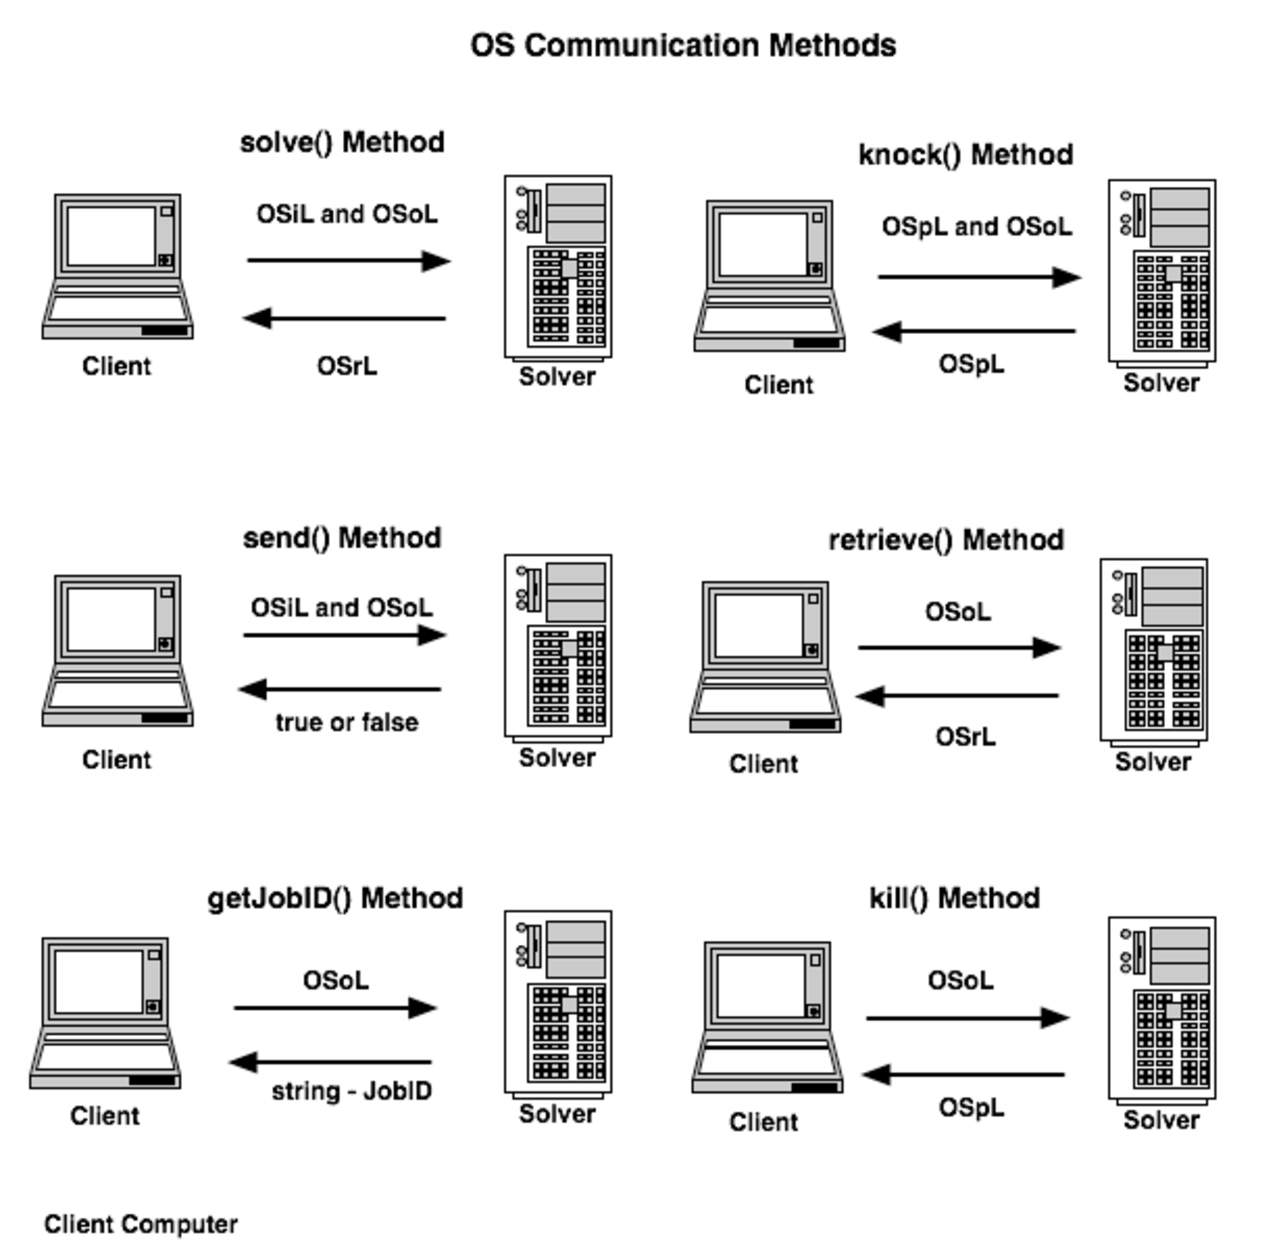
\includegraphics[scale=0.5]{./figures/osCommunicationMethods.pdf}%
\lthtmlpictureZ
\lthtmlcheckvsize\clearpage}

\stepcounter{section}
\stepcounter{section}
\stepcounter{subsection}
\stepcounter{subsection}
{\newpage\clearpage
\lthtmlinlinemathA{tex2html_wrap_inline9166}%
$ <$%
\lthtmlinlinemathZ
\lthtmlcheckvsize\clearpage}

{\newpage\clearpage
\lthtmlinlinemathA{tex2html_wrap_inline9168}%
$ >$%
\lthtmlinlinemathZ
\lthtmlcheckvsize\clearpage}

{\newpage\clearpage
\lthtmlfigureA{verbatimtab2483}%
\begin{verbatimtab}[5]
<osol>
    <general>
         <instanceLocation locationType="local">
         	/home/kmartin/temp/parincQuadratic.osil
         </instanceLocation>
    </general>
    <optimization>
    	<other name="os_solver">ipopt</other>
    </optimization>
</osol>
\end{verbatimtab}%
\lthtmlfigureZ
\lthtmlcheckvsize\clearpage}

\stepcounter{section}
\stepcounter{subsection}
\stepcounter{subsection}
{\newpage\clearpage
\lthtmlinlinemathA{tex2html_wrap_inline9179}%
$ -100$%
\lthtmlinlinemathZ
\lthtmlcheckvsize\clearpage}

{\newpage\clearpage
\lthtmlinlinemathA{tex2html_wrap_inline9181}%
$ 100$%
\lthtmlinlinemathZ
\lthtmlcheckvsize\clearpage}

{\newpage\clearpage
\lthtmlinlinemathA{tex2html_wrap_inline9185}%
$ x_{0}*x_{1}$%
\lthtmlinlinemathZ
\lthtmlcheckvsize\clearpage}

\stepcounter{subsection}
\stepcounter{section}
\stepcounter{subsection}
{\newpage\clearpage
\lthtmlinlinemathA{tex2html_wrap_inline9190}%
$ x_i$%
\lthtmlinlinemathZ
\lthtmlcheckvsize\clearpage}

{\newpage\clearpage
\lthtmlinlinemathA{tex2html_wrap_inline9192}%
$ i$%
\lthtmlinlinemathZ
\lthtmlcheckvsize\clearpage}

{\newpage\clearpage
\lthtmlinlinemathA{tex2html_wrap_inline9194}%
$ =$%
\lthtmlinlinemathZ
\lthtmlcheckvsize\clearpage}

{\newpage\clearpage
\lthtmlinlinemathA{tex2html_wrap_inline9196}%
$ \ge$%
\lthtmlinlinemathZ
\lthtmlcheckvsize\clearpage}

{\newpage\clearpage
\lthtmlinlinemathA{tex2html_wrap_indisplay9199}%
$\displaystyle x_{1} + x_{2} + x_{3}$%
\lthtmlindisplaymathZ
\lthtmlcheckvsize\clearpage}

{\newpage\clearpage
\lthtmlinlinemathA{tex2html_wrap_indisplay9203}%
$\displaystyle 1$%
\lthtmlindisplaymathZ
\lthtmlcheckvsize\clearpage}

{\newpage\clearpage
\lthtmlinlinemathA{tex2html_wrap_indisplay9205}%
$\displaystyle 0.3221 x_{1} +   0.0963x_{2} +    0.1187x_{3}$%
\lthtmlindisplaymathZ
\lthtmlcheckvsize\clearpage}

{\newpage\clearpage
\lthtmlinlinemathA{tex2html_wrap_indisplay9207}%
$\displaystyle \ge$%
\lthtmlindisplaymathZ
\lthtmlcheckvsize\clearpage}

{\newpage\clearpage
\lthtmlinlinemathA{tex2html_wrap_indisplay9209}%
$\displaystyle .15$%
\lthtmlindisplaymathZ
\lthtmlcheckvsize\clearpage}

{\newpage\clearpage
\lthtmlinlinemathA{tex2html_wrap_indisplay9212}%
$\displaystyle \min  0.4253 x_{1}^{2} +  0.4458 x_{2}^{2} + 0.2314 x_{3}^{2} + 2 \times 0.1852 x_{1} x_{2}$%
\lthtmlindisplaymathZ
\lthtmlcheckvsize\clearpage}

{\newpage\clearpage
\lthtmlinlinemathA{tex2html_wrap_indisplay9214}%
$\displaystyle + 2 \times 0.1393 x_{1} x_{3} + 2 \times
0.1388 x_{2} x_{3}$%
\lthtmlindisplaymathZ
\lthtmlcheckvsize\clearpage}

{\newpage\clearpage
\lthtmlinlinemathA{tex2html_wrap_inline9216}%
$ Q$%
\lthtmlinlinemathZ
\lthtmlcheckvsize\clearpage}

\stepcounter{subsection}
{\newpage\clearpage
\lthtmlfigureA{verbatimtab2604}%
\begin{verbatimtab}[5]
<?xml version="1.0" encoding="UTF-8"?>
<osil xmlns="os.optimizationservices.org">
	<instanceHeader>
		<name>Modified Rosenbrock</name>
		<source>Computing Journal 3:175-184, 1960</source>
		<description>Rosenbrock problem with constraints</description>
	</instanceHeader>
	<instanceData>
		<variables numberOfVariables="2">
			<var lb="0" name="x0" type="C"/>
			<var lb="0" name="x1" type="C"/>
		</variables>
		<objectives numberOfObjectives="1">
			<obj maxOrMin="min" name="minCost" numberOfObjCoef="1">
				<coef idx="1">9.0</coef>
			</obj>
		</objectives>
		<constraints numberOfConstraints="2">
			<con ub="25.0"/>
			<con lb="10.0"/>
		</constraints>
		<linearConstraintCoefficients numberOfValues="3">
			<start>
				<el>0</el><el>2</el><el>3</el>
			</start>
			<rowIdx>
				<el>0</el><el>1</el><el>1</el>
			</rowIdx>
			<value>
				<el>1.</el><el>7.5</el><el>5.25</el>
			</value>
		</linearConstraintCoefficients>
		<quadraticCoefficients numberOfQuadraticTerms="3">
			<qTerm idx="0" idxOne="0" idxTwo="0" coef="10.5"/>
			<qTerm idx="0" idxOne="1" idxTwo="1" coef="11.7"/>
			<qTerm idx="0" idxOne="0" idxTwo="1" coef="3."/>
		</quadraticCoefficients>
\end{verbatimtab}%
\lthtmlfigureZ
\lthtmlcheckvsize\clearpage}

{\newpage\clearpage
\lthtmlfigureA{verbatimtab2606}%
\begin{verbatimtab}[5]
		<nonlinearExpressions numberOfNonlinearExpressions="2">
			<nl idx="-1">
				<plus>
					<power>
						<minus>
							<number type="real" value="1.0"/>
							<variable coef="1.0" idx="0"/>
						</minus>
						<number type="real" value="2.0"/>
					</power>
					<times>
						<power>
							<minus>
								<variable coef="1.0" idx="0"/>
								<power>
									<variable coef="1.0" idx="1"/>
									<number type="real" value="2.0"/>
								</power>
							</minus>
							<number type="real" value="2.0"/>
						</power>
						<number type="real" value="100"/>
					</times>
				</plus>
			</nl>
			<nl idx="1">
				<ln>
					<times>
						<variable coef="1.0" idx="0"/>
						<variable coef="1.0" idx="1"/>
					</times>
				</ln>
			</nl>
		</nonlinearExpressions>
	</instanceData>
</osil>
\end{verbatimtab}%
\lthtmlfigureZ
\lthtmlcheckvsize\clearpage}

\stepcounter{subsection}
{\newpage\clearpage
\lthtmlfigureA{verbatimtab2612}%
\begin{verbatimtab}
<?xml version="1.0" encoding="UTF-8"?>
<osil  xmlns="os.optimizationservices.org"
     xmlns:xsi="http://www.w3.org/2001/XMLSchema-instance"
     xsi:schemaLocation="os.optimizationservices.org
     http://www.optimizationservices.org/schemas/OSiL.xsd">
	<instanceHeader>
		<description>A test problem for Algorithmic Differentiation</description>
	</instanceHeader>
	<instanceData>
		<variables numberOfVariables="4">
			<var lb="0" name="x0" type="C"/>
			<var lb="0" name="x1" type="C"/>
			<var lb="0" name="x2" type="C"/>
			<var lb="0" name="x3" type="C"/>
		</variables>
		<objectives numberOfObjectives=" 1">
			<obj maxOrMin="min" name="minCost" numberOfObjCoef="1">
				<coef idx="1">9.0</coef>
			</obj>
		</objectives>
		<constraints numberOfConstraints="2">
			<con ub="10.0" constant="33"/>
			<con lb="10.0"/>
		</constraints>
		<linearConstraintCoefficients numberOfValues="2">
			<start>
				<el>0</el>
				<el>0</el>
				<el>1</el>
				<el>2</el>
				<el>2</el>
			</start>
			<rowIdx>
				<el>0</el>
				<el>1</el>
			</rowIdx>
			<value>
				<el>5</el>
				<el>7</el>
			</value>
		</linearConstraintCoefficients>
		<nonlinearExpressions numberOfNonlinearExpressions="3">
			<nl idx="1">
				<ln>
					<times>
						<variable coef="1.0" idx="0"/>
						<variable coef="1.0" idx="3"/>
					</times>	
				</ln>
			</nl>
			<nl idx="0">
				<sum>
					<number type="real" value="-105"/>
					<variable coef="1.37" idx="1"/>
					<variable coef="2" idx="3"/>
				</sum>	
			</nl>
			<nl idx="-1">
				<power>
					<variable coef="1.0" idx="0"/>
					<number type="real" value="2.0"/>
				</power>
			</nl>
		</nonlinearExpressions>
	</instanceData>
</osil>
\end{verbatimtab}%
\lthtmlfigureZ
\lthtmlcheckvsize\clearpage}


\end{document}
